\documentclass{beamer}
\usepackage{graphicx}
\usepackage{hyperref}

\title{Towards Real-Time Physics in a 2D Survival-Based Game}
\author{Björn Aheimer, Felix Röhr, Daniel Six, Aleksis Vezenkov, Anietta Weckauff}
\date{University of Stuttgart, 2024}

\begin{document}

\begin{frame}
    \titlepage
\end{frame}

\begin{frame}{Introduction}
    \begin{itemize}
        \item Project objective: Enhance "Surviving Sarntal" with modular code, real-time physics, and improved user experience.
        \item Key areas of focus:
        \begin{itemize}
            \item Game engineering principles
            \item Modular structure
            \item Robust, efficient physics engine
        \end{itemize}
    \end{itemize}
\end{frame}

\begin{frame}{The Game Concept}
    \begin{itemize}
        \item Endless runner game focused on survival.
        \item Player controls a hiker who must dodge rocks and survive as long as possible.
        \item Collect items along the way to gain health, protection, or other benefits.
    \end{itemize}
\end{frame}

\begin{frame}{Project Enhancements}
    \begin{itemize}
        \item Transitioned from ECS to OOP for code modularity and maintainability.
        \item Comprehensive graphics overhaul for terrain, entities, and backgrounds.
    \end{itemize}
    \begin{figure}
        \centering
        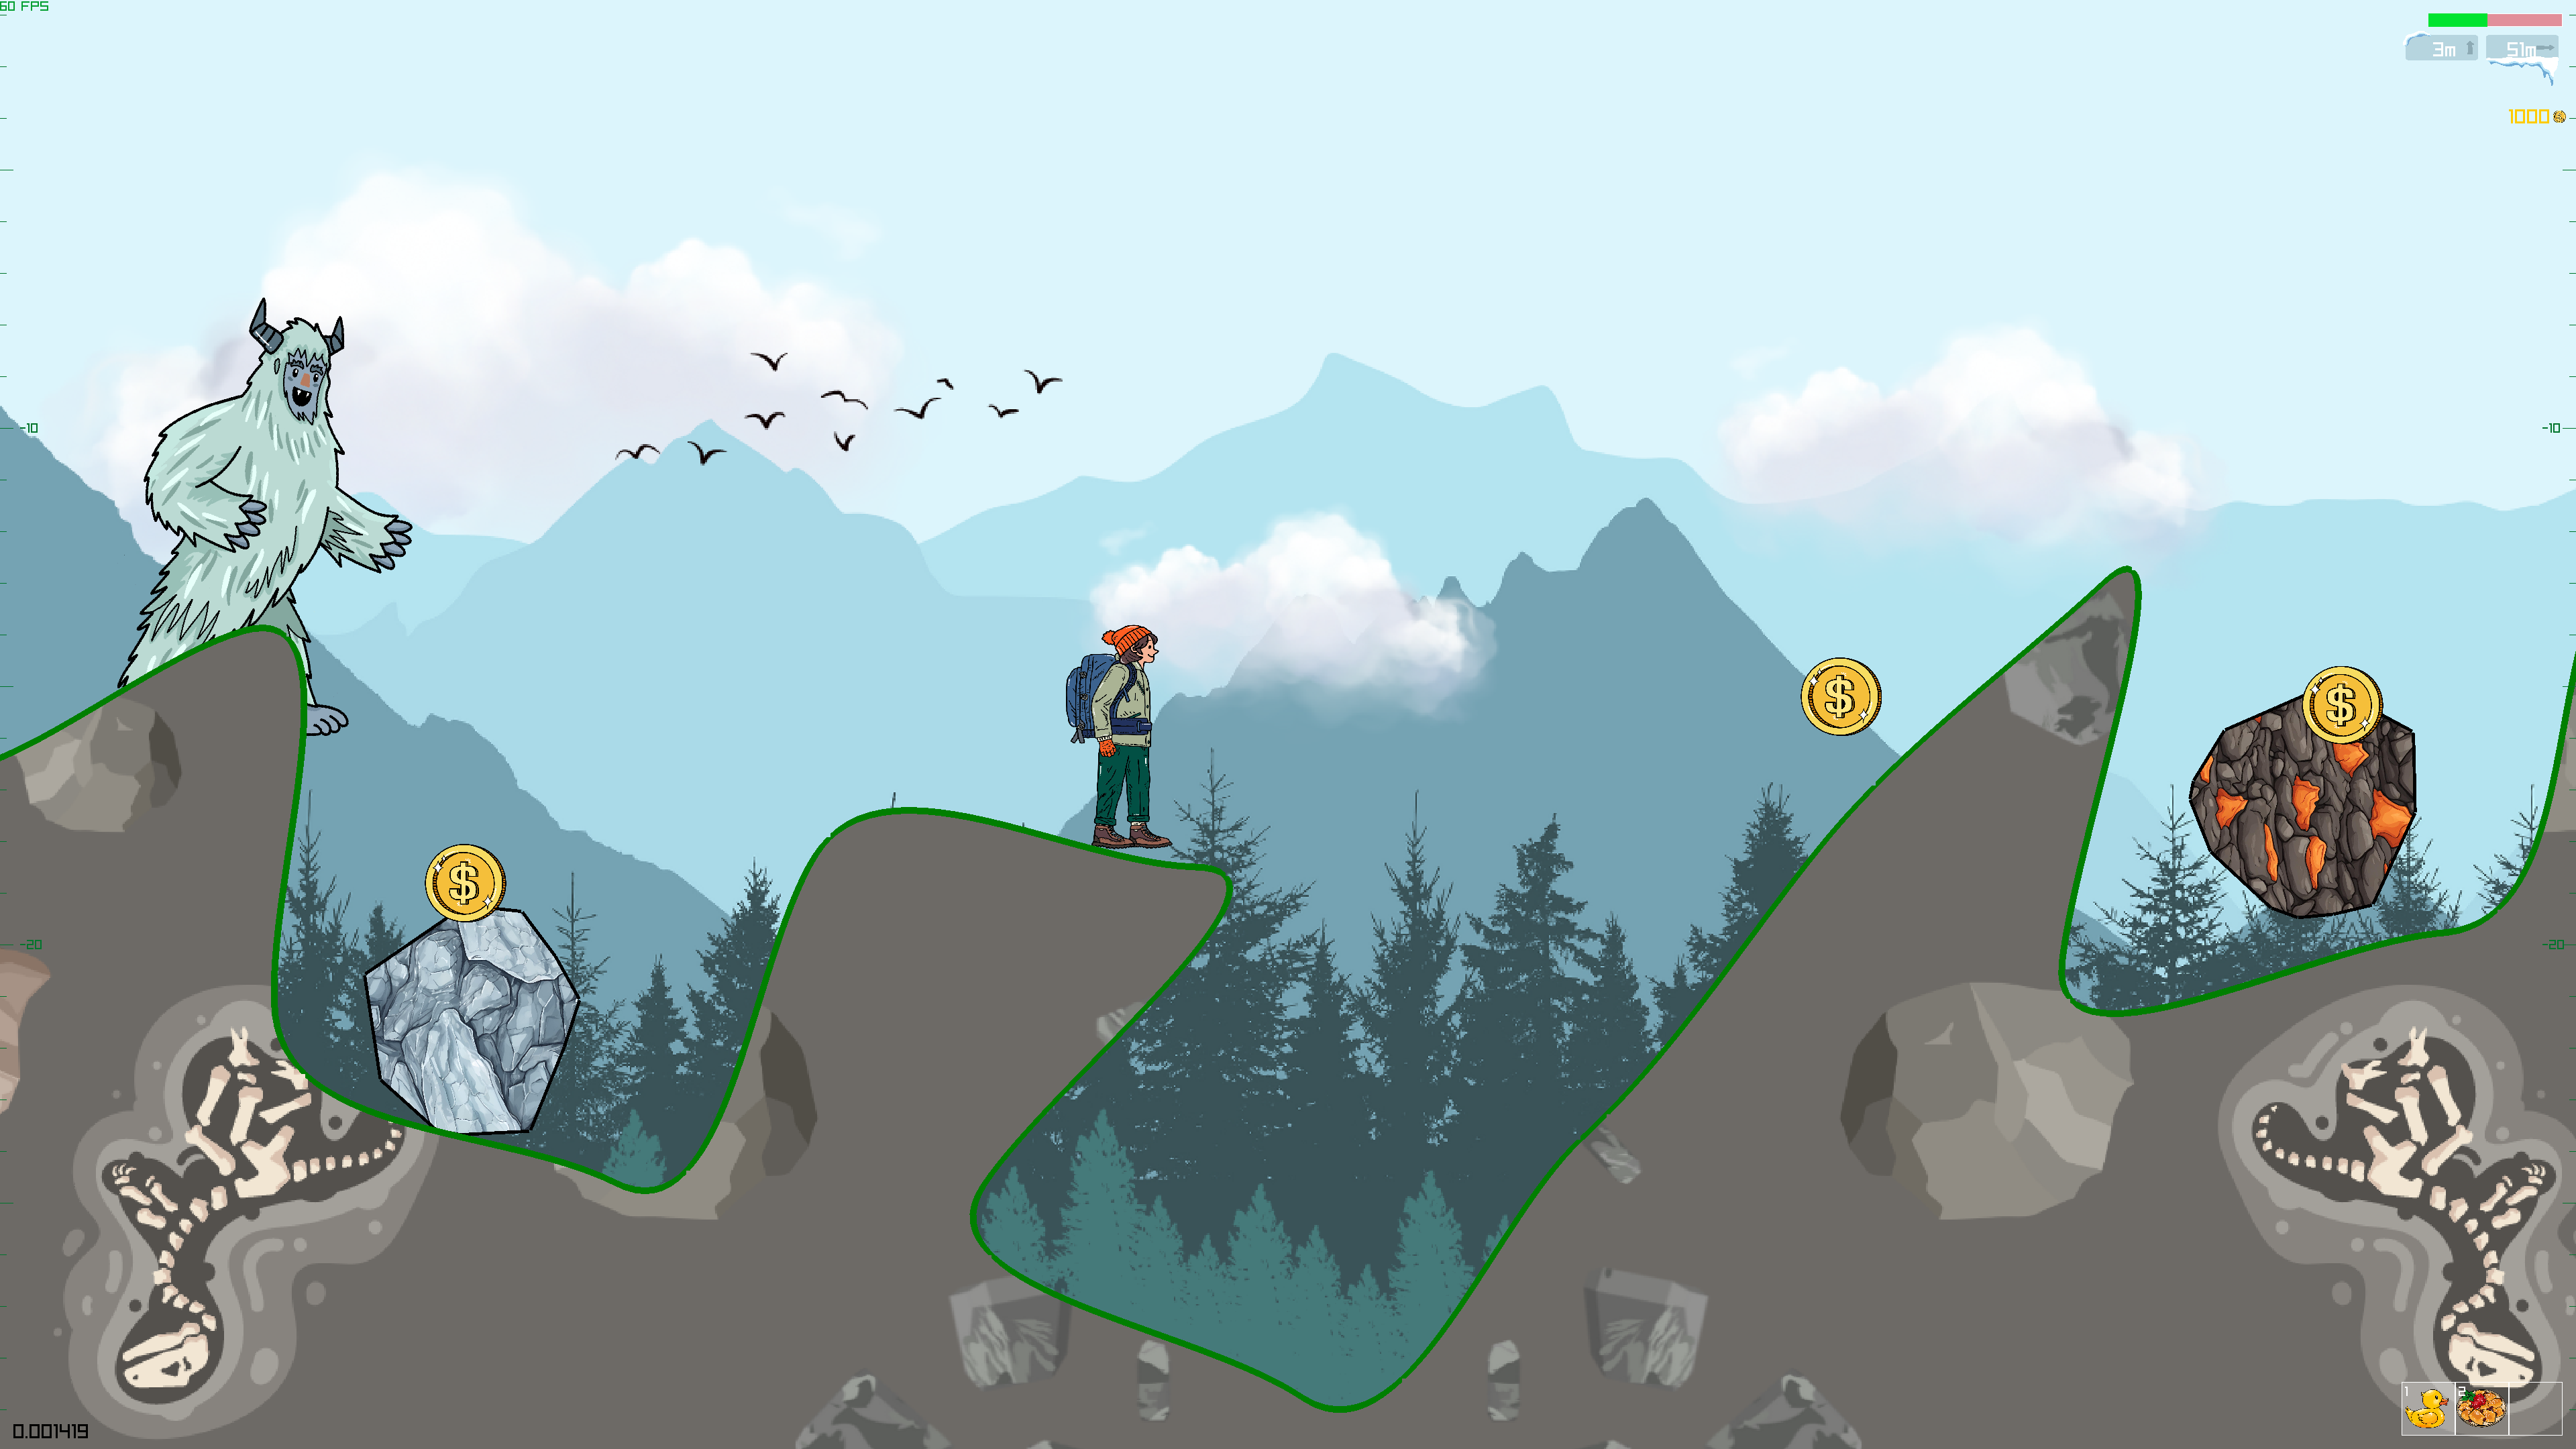
\includegraphics[width=0.6\textwidth]{../figures/new_game.png} % Insert new game screenshot here
        \caption{Enhanced graphics in the new version}
    \end{figure}
\end{frame}

\begin{frame}{Game Architecture}
    \begin{itemize}
        \item Modular design with distinct components for input, physics, rendering, and more.
        \item Game loop structured around core phases:
        \begin{itemize}
            \item Input handling
            \item Physics updates
            \item Rendering updates
        \end{itemize}
    \end{itemize}
    \centering
    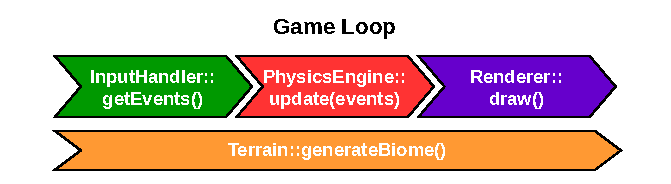
\includegraphics[width=0.6\textwidth]{../figures/physics/gameLoop.pdf} % Insert game loop diagram
\end{frame}

\begin{frame}{Physics Engine}
    \begin{itemize}
        \item Designed to enable real-time physics without compromising performance.
        \item Frame rate and physics rate are decoupled to maintain fluid gameplay.
        \item Key components:
        \begin{itemize}
            \item Collision detection and handling
            \item Rigid body dynamics simulation
        \end{itemize}
    \end{itemize}
\end{frame}

\begin{frame}{Collision Detection and Resolution}
    \begin{itemize}
        \item Uses Separating Axis Theorem (SAT) to detect collisions between convex shapes.
        \item Optimizations with swept axis-aligned bounding boxes (AABBs) to enhance accuracy.
        \item Collision depth-based resolution to ensure stability during gameplay.
    \end{itemize}
    \centering
    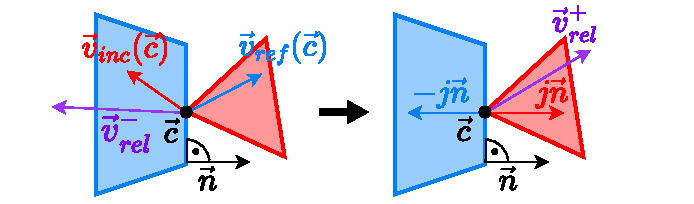
\includegraphics[width=0.6\textwidth]{../figures/physics/resolution.pdf} % Insert collision detection diagram
\end{frame}

\begin{frame}{Terrain Generation}
    \begin{itemize}
        \item Terrain is generated using Hermite splines for smooth 2D paths.
        \item Procedurally generated biomes that adapt as the player progresses.
        \item Constraints ensure terrain is navigable without intersecting or backward generation.
    \end{itemize}
    \centering
    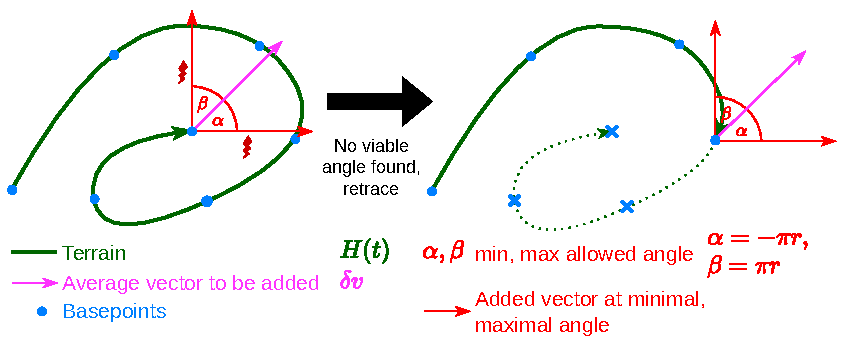
\includegraphics[width=0.6\textwidth]{../figures/Retrace.pdf} % Insert terrain generation diagram
\end{frame}

\begin{frame}{Rendering Architecture}
    \begin{itemize}
        \item Central Renderer class with sub-renderers for different game elements:
        \begin{itemize}
            \item Terrain, Entities, HUD
        \end{itemize}
        \item Real-time rendering with camera effects like shake and dynamic zoom.
        \item Debug mode enables hitbox and terrain triangulation visualization for development.
    \end{itemize}
\end{frame}

\begin{frame}{Performance Considerations}
    \begin{itemize}
        \item Performance optimizations for handling large numbers of entities.
        \item Sub-stepping for fast-moving objects to enhance collision accuracy.
        \item Effective garbage collection for entities and terrain that leave the active area.
    \end{itemize}
\end{frame}

\begin{frame}{Conclusion and Future Work}
    \begin{itemize}
        \item Achievements:
        \begin{itemize}
            \item Modular architecture and optimized codebase
            \item Enhanced user experience with new features
        \end{itemize}
        \item Proposed future expansions:
        \begin{itemize}
            \item Multiplayer modes and leaderboard integration
            \item New game items and biomes
            \item Enhanced physics with friction, air resistance, and more
        \end{itemize}
    \end{itemize}
\end{frame}

\begin{frame}
    \centering
    \Huge Thank You! \\
    \vspace{1cm}
    \Large Questions?
\end{frame}

\end{document}
